\documentclass[11pt,a4paper,twoside,openright]{report}
\usepackage[english]{babel}
\usepackage[utf8]{inputenc}
\usepackage[T1]{fontenc}
\usepackage{amsmath}
\usepackage{amsfonts}
\usepackage{amssymb}
\usepackage{amstext}
\usepackage{booktabs}
\usepackage{csquotes}
\usepackage{epigraph}
\usepackage{geometry}%\geometry{hmargin=2.5cm, vmargin=2.5cm}
\usepackage{lmodern}
\usepackage{listings}
\usepackage{gensymb}
\usepackage{textcomp}
\usepackage{titlesec}
\usepackage{graphics}
\usepackage[pdftex]{graphicx}
\usepackage{tikz}
\usetikzlibrary{automata,arrows,positioning,shapes}
\usepackage{tikz-qtree}
\usepackage{pgfplots}
\usepackage{url}
%\usepackage{hyperref}
\usepackage[pdftex,
            pdfauthor={Nathan Magrofuoco},
            pdftitle={Conception, design and testing of a split menu for 
smartphone}]{hyperref}
\usepackage{setspace}
\usepackage{cite}
\usepackage{pdfpages}
\usepackage{array}
\usepackage{wrapfig}
\usepackage{ccaption}
\usepackage{subcaption}
\usepackage{appendix}
\usepackage{textcomp}
\usepackage[official]{eurosym}
%Centre les caption de plus d'une ligne sous la figure
\usepackage[justification=centering]{caption}% or e.g. [format=hang]
%\usepackage[]{mcode} %Matlab
\usepackage{colortbl}
\usepackage{longtable}
\usepackage{multirow}
\usepackage{xcolor}
%\usepackage{verbatim}
\usepackage{fancyhdr} %Stype de page

%Matlab to latex
\usepackage[framed,numbered,autolinebreaks,useliterate]{mcode}

\fancyhead[L]{\begin{tabular}{|p{33mm}}\hline\rowcolor[rgb]{0,0,0.5}\textcolor{
white}{\small\bf\docsigle}\\\hline\small\bf\docversion\\\hline\end{tabular}}
\fancyhead[C]{\begin{tabular}{p{9cm}c}\hline\rowcolor[rgb]{0,0,0.5}
\centering\textcolor{white}{\bf\small\doctitle}&\\\hline\space 
&\\\hline\end{tabular}}

\renewcommand{\thesection}{\arabic{section}}

\fancyfoot[L]{}
\fancyfoot[C]{}
\fancyfoot[R]{\textcolor[gray]{0.4}{Page \thepage~sur~\pageref{LastPage}}}

\renewcommand{\headrulewidth}{0pt}
\renewcommand{\footrulewidth}{0pt}

%%%% debut macro marge locale %%%%
\newenvironment{changemargin}[2]{\begin{list}{}{%
\setlength{\topsep}{0pt}%
\setlength{\leftmargin}{0pt}%
\setlength{\rightmargin}{0pt}%
\setlength{\listparindent}{\parindent}%
\setlength{\itemindent}{\parindent}%
\setlength{\parsep}{0pt plus 1pt}%
\addtolength{\leftmargin}{#1}%
\addtolength{\rightmargin}{#2}%
}\item }{\end{list}}
%%%% fin macro %%%%

\usepackage{tabularx}
\usepackage{algorithmic}


%%Filigrane de confidentialite
%\usepackage{draftwatermark}
%\SetWatermarkLightness{0.8}
%\SetWatermarkAngle{25}
%\SetWatermarkScale{2}
%\SetWatermarkFontSize{2cm}
%\SetWatermarkText{Confidentiel}


%\newcommand{\myheading}[1]{\hspace{-1em}\textbf{#1}\\}
\newcommand{\HRule}{\rule{\linewidth}{0.5mm}}

\author{Nathan Magrofuoco}

\makeindex

\begin{document}

\setstretch{1.3} % Line spacing of 1.3

\includepdf[pages={1-2}]{cover/cover.pdf}

\thispagestyle{empty}
\epigraph{\enquote{It is far better to adapt the technology to the user than to 
force the user to adapt to the technology.}}{\textit{Larry Marine}}
\null\newpage
\thispagestyle{empty}

\null\newpage

\pagenumbering{roman}
\chapter*{Acknowledgements}

This Master's thesis is the accomplishment of many years of ongoing learning. 
It represents my contribution to this magnificent field of study which is 
human-computer interaction.\\

I would first like to thank sincerely my thesis advisor Prof. Jean
\textsc{Vanderdonckt}. His door was always open whenever I ran into an issue 
or had a question about my research or experiment. He steered me in the 
right direction from our first meeting until the very last one. Even though he 
was travelling or on vacation, he was always careful about my doubts and 
questions.\\

I would also like to acknowledge the participants of the experiment. They 
graciously agreed to take part to this thesis by giving their free time to 
computer science.\\

Finally, I must express my very profound gratitude to my parents for 
providing me with unfailing support and continuous encouragement throughout my 
own process of learning, studying, researching, coding and writing this 
thesis. This accomplishment would not have been possible without them. Thank 
you.\\

\begin{flushright}
Nathan \textsc{Magrofuoco}
\end{flushright}

\null\newpage
\chapter*{Abstract}
In 1994, \textsc{Sears} and \textsc{Shneiderman} proposed the changing concept 
of split menu. They have radically influenced the way we have designed menus 
until today. Unfortunately, their guidelines haven't evolved in 20 years and 
the advent of smartphones have led HCI researchers to new and different 
usability issues. Based on their initial study, this master thesis aims to 
conceive, design and test a split menu adapted to smartphone 
resolutions.\newline

Along the way, the approaches from various researchers have influenced our 
experiment and diverse menu organizations have also been designed and tested. 
An experimental method has been conducted combining traditional, split, 
responsive, minimised and mixed-initiative menus. The objective of this method 
was to assess the usability of these new menu organizations on smartphones. 
Usability has been studied along with 3 interesting properties: (1) 
effectiveness, (2) efficiency and (3) user satisfaction.\newline

The experiment proved that split menu may not be the ideal solution for 
smartphones. Another novative menu organization called \enquote{responsive} 
has shown a better usability. This dissertation aims to explain the development 
of the experiment and argue the analysis of its results.

\cleardoublepage
\tableofcontents
% \lhead{\emph{List of Figures}}
% \listoffigures
% \lhead{\emph{List of Tables}}
% \listoftables

\cleardoublepage
\pagenumbering{arabic}
\chapter{Introduction}
Since the initial drawings of Charles \textsc{Babbage} and the first modern 
computer 
built by Konrad \textsc{Zuse}, computer technology has widely evolved and 
spread around 
the globe. Initially dedicated and used by a few IT professionals, 
the advent of personal computing radically changed the game and made everyone a 
potential computer user \cite{hci}. Computer providers faced serious usability 
issues with the initial command dialogs. Some still recognized brands took 
advantage of innovative and creative minds to overcome these problems.\newline

Unfortunately the effectiveness of their solutions has often not been 
scientifically proven. In the early 1980s, some computer scientists showed 
great 
interest into assessing the usability of the traditionally designed UI's. An 
area of research and practice called \enquote{\textit{human-computer 
interaction}} - and 
commonly referred to as \textit{HCI} - started to emerge along with these 
scientists. They focused on studying the quality and quantity of information 
transfer between humans and computers. Later they started to publish their own 
mathematical models and related UI solutions to enhance UX.\newline

Last decade saw the rise of mobile technologies. Minimising computer components 
has always been a common interest for computer manufacturers. Smartphone in the 
hand, tablet in the other. People have become keen of these microtechnologies. 
Unfortunately they raised new issues. Among them, the complexification of UI has 
become an increasing problem for users, especially for novices. We come to a 
point where humans themselves must adapt to the technology and HCI has still a 
long road ahead.

\section{Objectives}
This master thesis was initially focused on the conception, the design and the 
testing of a split menu for smartphone. Starting with the guidelines proposed 
by \textsc{Sears} and \textsc{Shneiderman} \cite{sears} almost 20 years ago, the 
first objective 
was to design a \textit{usable} split menu in the context of a small 
touching screen. Assessing \textit{usability} requires to be attentive to 3 
interesting properties : (1) effectiveness, (2) efficiency and (3) 
satisfaction. A controlled experiment was planned to be conducted in order to 
evaluate these properties and compare a traditional menu organization to a 
split menu designed for smartphone. \newline

The conception and the design of such a split menu also required to update the 
guidelines published by \textsc{Sears} and \textsc{Shneiderman}. Indeed these 
guidelines haven't been modified since 1994. An intense review of the field of 
study brang us to take into account diverse 
approaches. Many researchers and studies have therefore influenced the conducted 
experiment. The master thesis is finally more about conceiving, designing and 
testing new menu organizations for smartphone.

\section{Structure of the written dissertation}
The written dissertation is organized as follows:

\begin{enumerate}
  \item \textbf{State of the Art}: the first chapter is the starting point of 
the study. It provides a review of the field of research and describes the 
knowledge base over which the entire experiment was built.
  \item \textbf{Methodology}: the second chapter describes the methodology used 
to conceive the experiment. First, it presents the initial hypotheses. Then, it 
describes the experimental method. Finally it argues the Android app used 
during the study.
  \item \textbf{Results}: the third chapter provides an overview of the results 
gathered during the experiment, then it analyzes these results to 
confirm, reverse and update the initial hypotheses.
  \item \textbf{Conclusion}: finally, a conclusion ends the written 
dissertation by discussing the confirmed hypotheses, the encoutered issues, 
the unchallenged matters and the future improvements to be made.
\end{enumerate}



\input{state_of_art.tex}
\chapter{Methodology}
The methodology is mainly inspired by the previous researches described in the 
state of the art. A set of 11 hypotheses are described and argued based on the 
learning outcomes of the previous chapter. Then, the experimental method that 
aims to confirm or reverse these hypotheses is deeply reviewed. Finally, the 
related implementation is reported for computer scientists’ interests.

\section{Hypotheses} \label{hypotheses}
A set of 11 hypotheses have been initially formulated. Each hypothesis is based 
on one or several learning outcomes from one or several researchers. The 
objective is to study the field of research even further than the previous 
experiments. The hypotheses will be later confirmed or reversed by the 
experiment. Some new hypotheses may even be formulated afterwards with respect 
to the results of the experiment.

\begin{itemize}
 \item \textbf{H1a:} the split menu reduces the selection time.
 \item \textbf{H1b:} the split menu is preferred 
by users.
\end{itemize}

\textsc{Sears} and \textsc{Shneiderman} proved that a split menu following a 
strict set of 
guidelines could be beneficial for both user experience and user performance. 
Therefore, a menu providing a hot list of items based on frequency reordering 
should indeed reduce selection time and receive a higher user 
preference.

\begin{itemize}
  \item \textbf{H2a:} the minimised menu reduces the selection time.
  \item \textbf{H2b:} the minimised menu is preferred by users.
\end{itemize}

Khalid \textsc{Al-Omar} and Dimitrios \textsc{Rigas} identified a clear user 
preference for their minimised menu. Such a menu hides unwanted items and 
therefore reduces the number of items displayed on the screen. This is very 
related to the \textit{rules of ergonomy} taught by Professor Jean Vanderdonckt 
in his course entitled \enquote{human-computer interaction} at Univeristé 
Catholique de Louvain (BE). One HCI rule called \enquote{rule of thumb} states 
that an interface should display a minimum of 4 items and a maximum of 8. 
Unfortunately, this rule is still neglected by the researchers. The idea is to 
implement a menu which displays a restricted number of items at the same time. 
It should be easier to read and manipulate for users, especially for novice 
ones.

\begin{itemize}
  \item \textbf{H3a:} the responsive menu reduces the selection time.
  \item \textbf{H3b:} the responsive menu is preferred by users.
\end{itemize}

Yusuke \textsc{Fukazawa} studied the effects of menu organization with a 
specific focus towards small mobile screens. He proved that a responsive menu 
organization could be beneficial for user experience. Unfortunately, his work 
must still be argued by further experiments. Since this master thesis aims to 
conceive and design a menu organization for smartphone, it is necessary to 
include his findings in the experimental method. Therefore, a responsive menu 
should be designed and tested.

\begin{itemize}
  \item \textbf{H4a:} novice users show a preference for the adaptive menus.
  \item \textbf{H4b:} master users show a preference for the traditional menu.
\end{itemize}

Yusuke \textsc{Fukazawa} found out that \textit{master users} preferred to have 
more 
control over menu customization and preferred to be less guided by the system. 
Therefore, they showed higher preferences for traditional and adaptable menus 
because they are respectively use to it and user-controlled. Our experiment is 
mainly focused towards adaptive menus and master users should therefore show a 
preference for traditional menu organizations only. At the opposite, 
\textit{novice users} showed higher preferences for adaptive menus which prove 
the system ability to handle menu customization by itself. They should show the 
same preferences during our experiment.

\begin{itemize}
  \item \textbf{H5a:} guidance informations help users to understand how a 
menu 
works.
  \item \textbf{H5b:} guidance informations help users to handle a menu more 
efficiently.
  \item \textbf{H5c:} a period of adjustment helps users to handle a menu more 
efficiently.
\end{itemize}

Khalid \textsc{Al-Omar} and Dimitrios \textsc{Rigas} proved that users needed 
both \textit{guidance informations} and a \textit{period of adjustment} in 
order to handle and understand new menu organizations, especially for adaptable 
menus. The experiment should however provide the same results for adaptive menus 
since they still represent new menu organizations for users. Notice that 
\textsc{Somberg}, and \textsc{Sears} and \textsc{Shneiderman} also observed 
that a period of adjustment was beneficial for user performance during their 
respective experiments.

\section{Experimental method}
The experimental method aims to confirm or reverse the hypotheses. In 
order to achieve this objective, 8 menu organizations have been designed and 
implemented in an Android application developed especially for the 
experiment. This subsection argues the choices performed during the development 
of the experimental method. It also describes its overall operation.

\subsection{Test protocol} \label{test_protocol}
Participants were first asked to answer a preliminary set of sociodemograhic 
questions on a survey paper. In order to prevent users from being distracted 
by a second computer screen, it was decided to use a paper version of the 
survey. It is available at the end of the dissertation, see Appendix 
\ref{survey}. The users were then asked to perform 2 kinds of sessions on the 
Android application. The first sessions were called 
\textit{training sessions} - or \textit{adjustment periods} in reference to 
\textsc{Somberg}' study \cite{somberg}. Each training session last for 2 
consecutive selections and was preceded by guidance informations. For each 
selection, the system randomly chose an item and displayed it on the screen. 
Once the menu was displayed, the participant had to press on the 
required item. Guidance informations were used to help users to understand the 
following menu organization. A second set of sessions was organized after the 8 
training sessions. These new sessions were called \textit{evaluation sessions} 
and last for 10 consecutive selections. An evaluation session was not preceded 
by guidance informations but was followed by a set of questions to answer on 
the survey paper. These questions were used to assess the usability of the menu 
organization and gather user's feedback. During the evaluation sessions, 6 
parameters were recorded for each selection: (1) the the required item, (2) 
its 
position in the menu, (3) the selected item, (4) its position in the menu, (5) 
the selection time and (6) the correctness of the selection.

\subsection{Items}
The items displayed by the Android application have been selected from a 
controlled experiment conducted by \textsc{Findlater} \cite{findlater}. This 
experiment 
used 16 items divided into 4 specific categories. Notice that Khalid 
\textsc{Al-Omar} and 
Dimitrios \textsc{Rigas} considered such a menu as a \textit{small} one during 
their own 
study \cite{alomar1}. Figure \ref{fig:items} depicts the categories of items 
described by \textsc{Findlater} and used during the experiment.\newline

\begin{figure}[!ht]
    \centering
    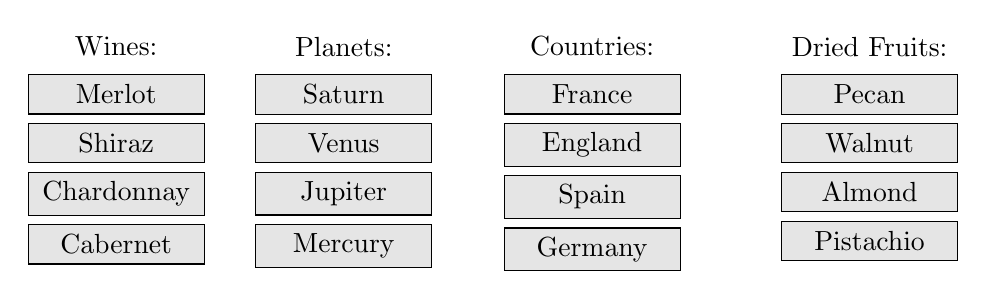
\begin{tikzpicture}[node distance=0.8cm]
        \tikzstyle{item}
	  =[draw, fill=gray!20, rectangle, text width=2cm, 
	  minimum height=0.5cm, text centered]
	
	\node[] (wines)
	  {Wines:};
	\node[item] (A)
	  [below=3pt of wines]{Merlot};
	\node[item] (B)
	  [below=3pt of A] {Shiraz};
	\node[item] (C)
	  [below=3pt of B] {Chardonnay};
	\node[item] (D)
	  [below=3pt of C] {Cabernet};
	  
	\node[] (planets)
	  [right=1.5cm of wines] {Planets:};
	\node[item] (cat11)
	  [below=3pt of planets] {Saturn};
	\node[item] (cat12)
	  [below=3pt of cat11] {Venus};
	\node[item] (cat21)
	  [below=3pt of cat12] {Jupiter};
	\node[item] (cat31)
	  [below=3pt of cat21] {Mercury};
	 
	\node[] (countries)
	  [right=1.5cm of planets]{Countries:};
	\node[item] (F2)
	  [below=3pt of countries] {France};
	\node[item] (D2)
	  [below=3pt of F2] {England};
	\node[item] (A2)
	  [below=3pt of D2] {Spain};
	\node[item] (C2)
	  [below=3pt of A2] {Germany};
	  
	\node[] (dried)
	  [right=1.5cm of countries]{Dried Fruits:};
	\node[item] (F3)
	  [below=3pt of dried] {Pecan};
	\node[item] (D3)
	  [below=3pt of F3] {Walnut};
	\node[item] (A3)
	  [below=3pt of D3] {Almond};
	\node[item] (C3)
	  [below=3pt of A3] {Pistachio};
    \end{tikzpicture}
    \caption{The 4 categories of 4 items described by \textsc{Findlater} and 
used 
during the experiment.}
    \label{fig:items}
\end{figure}

\subsection{Control condition menu}
A control condition menu stands as baseline to perform the comparison between a 
set of menu organizations. For this experiment, a traditional vertical menu 
was chosen to be the control condition menu. It consisted of a 1-column menu 
which displayed the items in categorical order such that wines were grouped 
together, followed by planets, countries and dried fruits in the order 
displayed 
by Figure \ref{fig:items}.
%The control 
%condition menu organization is depicted by Figure \ref{fig:control_menu}.

% \begin{figure}[!ht]
%     \centering
    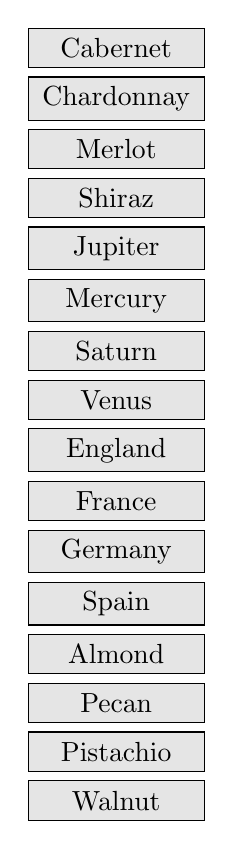
\begin{tikzpicture}[node distance=0.8cm]
        \tikzstyle{item}
	  =[draw, fill=gray!20, rectangle, text width=2cm, 
	  minimum height=0.5cm, text centered]

	\node[item] (A)
	  {Cabernet};
	\node[item] (B)
	  [below=3pt of A] {Chardonnay};
	\node[item] (C)
	  [below=3pt of B] {Merlot};
	\node[item] (D)
	  [below=3pt of C] {Shiraz};
	\node[item] (E)
	  [below=3pt of D] {Jupiter};
	\node[item] (F)
	  [below=3pt of E] {Mercury};
	\node[item] (G)
	  [below=3pt of F] {Saturn};
	\node[item] (H)
	  [below=3pt of G] {Venus};
	\node[item] (I)
	  [below=3pt of H] {England};
	\node[item] (J)
	  [below=3pt of I] {France};
	\node[item] (K)
	  [below=3pt of J] {Germany};
	\node[item] (L)
	  [below=3pt of K] {Spain};
	\node[item] (M)
	  [below=3pt of L] {Almond};
	\node[item] (N)
	  [below=3pt of M] {Pecan};
	\node[item] (O)
	  [below=3pt of N] {Pistachio};
	\node[item] (P)
	  [below=3pt of O] {Walnut};
    \end{tikzpicture}
    \caption{Control condition menu organization with the 16 items described by 
Findlater.}
%     \label{fig:control_menu}
% \end{figure}

\subsection{Split menu}
We followed the guidelines described by \textsc{Sears} and \textsc{Shneiderman} 
in order to 
confirm the hypotheses related to the split menu. Indeed, both authors defined 
a 
strict set of guidelines to design efficient split menus. As explained 
previously, these guidelines are based on 3 preliminary observations: (1) 
users know the name of the item they are looking for, (2) some items are 
more frequently selected than others and (3) these most frequent items are 
ideally not already located at the top of the menu. These preliminary 
observations are met during the experiment because users have to select items 
that are chosen and displayed by the system. \textsc{Sears} and 
\textsc{Shneiderman} developed 3 
guidelines based on these observations: (1) both the hot list and the 
traditional sections should respect the traditional ordering, (2) the hot list 
should not display more than 4 items and (3) the hot list should only display 
the most frequently selected items.\newline

For the experiment purpose, the hot list was decided to hold 3 items as 
\textsc{Findlater} used during his own study \cite{findlater}. The hot list was 
also 
decided to be highlighted. Therefore, the background of the hot list items was 
displayed in a dark blue colour called \textit{primary colour} in the initial 
Android theme.

\subsection{Minimised menu}
Traditional menus display the entire set of items at the same time. The users 
usually require to scroll down the menu to show the last items. Minimised menu 
aims to reduce the number of displayed items. Following the \textit{rule of 
thumb} described in the section \ref{hypotheses}, we designed a menu divided 
into consecutive and distinct \textit{pages}. Each page displays at most 8 
items. Since our initial set of items is made of 16 items, each menu 
organization is divided into 2 pages of exactly 8 items.

\subsection{Responsive menu}
The main objective of a responsive menu is to adapt the menu organization to 
the small size of mobile screens. The idea is to reduce both the size of 
displayed items and the margins in between these items. Sometimes it also 
consists of 
reducing the number of displayed items but we already implemented this 
opportunity with minimised menus. The responsive menu implemented for the 
experiment is designed with 2 columns of items. The first item is displayed in 
the top left column, the second one is displayed in the top right column and so 
on for the next items.

\subsection{Mixed-initiative menus}
Khalid \textsc{Al-Omar} and Dimitrios \textsc{Rigas} defined a 
\textit{mixed-initiative} menu as 
a menu that combines both adaptive and adaptable properties. During the 
experiment, a mixed-initiative menu was a menu organization combining split, 
minimised and/or responsive properties. Therefore 2x2x2 menu organizations have 
been designed to implement all the potential combinations of 
menus. These configurations are described in the following section and 
screenshots from the Android application are provided to better visualize the 
different menu organizations, see Appendix \ref{screenshots}.

\section{Implementation}
An Android application called \textit{Menuz} has been implemented to conduct 
the experiment. The application was responsible for displaying the menus and 
providing their guidance informations. It has also been designed to act as a 
guide during the experiment and therefore to give relevant directives to the 
participants. This subsection describes the architecture and choices performed 
during its implementation. Screenshots of the application are provided by 
Appendix \ref{screenshots}.

\subsection{Application architecture}
The Android application has been developed with \textit{Android Studio}. It is 
divided into 13 activities, 13 related XML layouts and Java classes, and one 
additional Java class for utility purpose. An android activity takes care of 
creating a window. It is first described by a XML layout in which Android 
components are assembled to form its UI. An additional Java class must also be 
implemented for each activity. This class allows to manage the activity 
lifecycle but also to react to user’s actions through listeners. Figure 
\ref{fig:activity} illustrates the concept of activity through the combination 
of an XML layout and a Java class.\newline

\begin{figure}[!ht]
    \centering
    \begin{tikzpicture}[node distance=0.8cm]
        \tikzstyle{file}
	  =[draw, rectangle, text width=2cm, minimum height=3cm, 
	  text centered]
	\tikzstyle{rect_xs}
	  =[draw, rectangle, text width=1.1cm, minimum height=.13cm, 
	  text centered]
	\tikzstyle{rect_xxs}
	  =[draw, rectangle, text width=0.7cm, minimum height=.1cm, 
	  text centered]
	  
	\node[file] (filexml) {};
	\node[] (xml) 
	  [above=3pt of filexml] {activity\_main.xml};
	\node[] (code1) 
	  [below left=9pt and -2.4cm of xml] {\_\_\_\_\_};
	\node[] (code2) 
	  [below left=3pt and -1.45cm of code1] {\_\_\_\_};
	\node[] (code3) 
	  [below left=3pt and -1.7cm of code2] {\_\_\_\_\_};
	\node[] (code4) 
	  [below left=3pt and -1.15cm of code3] {\_\_\_};
	\node[] (code5) 
	  [below left=3pt and -1.4cm of code4] {\_\_\_\_};
	  
	\node[file] (filejava)
	  [right=3cm of filexml] {};
	\node[] (java) 
	  [above=3pt of filejava] {MainActivity.java};
	\node[] (code6) 
	  [below left=9pt and -2.4cm of java] {\_\_\_\_\_};
	\node[] (code7) 
	  [below left=3pt and -1.45cm of code6] {\_\_\_\_};
	\node[] (code8) 
	  [below left=3pt and -1.7cm of code7] {\_\_\_\_\_};
	\node[] (code9) 
	  [below left=3pt and -1.15cm of code8] {\_\_\_};
	\node[] (code10) 
	  [below left=3pt and -1.4cm of code9] {\_\_\_\_};
	
	\node[inner sep=0, outer sep=0, draw=black, fill=black, 
	line width=0.06cm] (empty) 
	  [right=1.5cm of filexml] {};
	\node[] (empty1)
	  [below=1pt of empty] {};
	  
	\node[file] (windowfile)
	  [below=2.5cm of empty] {};
	\node[] (window) 
	  [above=3pt of windowfile] {window};
	\node[] (title)
	  [below=2.9cm of empty] {\_\_\_\_};
	\node[rect_xs] (textinput)
	  [below=3.8cm of empty] {};
	\node[rect_xxs] (button)
	  [below=4pt of textinput] {\_\_};
	
	\draw[-latex, line width=0.1cm] (empty)--(filexml);
	\draw[-latex, line width=0.1cm] (empty)--(filejava);
	\draw[-latex, dashed, line width=0.05cm] (empty1)--(window);
    \end{tikzpicture}
    \caption{An activity takes care of creating a window by combining a XML 
layout which defines its UI and a Java class which handles the activity 
lifecycle and user's actions.}
    \label{fig:activity}
\end{figure}

The entire application architecture is depicted by Figure 
\ref{fig:architecture}. The first activity is called \textit{MainActivity}. It 
welcomes the user and requires him to enter a username before starting the 
experiment. This first window is followed by an activity called 
\textit{IntroductionActivity} which introduces the course of the experiment. 
The 
user then receives the guidance informations of the first menu. Guidance 
informations are provided by an activity called 
\textit{MenuIntroductionActivity}. Its purpose is to introduce 
the new menu organizations to the subjects of the experiment. It leads to a 
fourth activity called \textit{NextSelectionActivity} which chooses a random 
item to be picked by the users. It also contains a selection counter to show 
the progress of the experiment. A selection timer starts when the participant 
presses on the \enquote{ready} button and once the menu has been entirely 
displayed on the screen. Each menu is designed to be a distinct activity. The 
activity is 
stopped when the user has performed a selection and the 
\textit{NextSelectionActivity} is called upon to display the next required item. 
The process is repeated until the 8 training sessions and the 8 evaluation 
sessions have been successfully achieved. Notice that a fifth activity called 
\textit{SurveyRequestActivity} is started at the end of each evaluation session 
to recall the user that he must answer a set of questions on the survey paper. 
During these evaluation sessions, \textit{MenuIntroductionActivity} doesn't 
display guidance informations anymore but acts as an intermediary window to 
announce the start of the next evaluation session. Finally, a class called 
\textit{Utility} has been implemented to allow developers to set up the 
experiment from one single file.\newline

\begin{figure}[!ht]
    \include{tikz/architecture}
    \label{fig:architecture}
\end{figure}

\subsection{Activities}
This second subsection describes the overal operation and the content of each 
activity and the additional \textit{Utility} class implemented in the Android 
application.

\subsubsection{MainActivity}
\textit{MainActivity.java} is the first activity called at the start of the 
application. The window is made of a \textit{TextView}, an \textit{EditText} 
and a \textit{Button}. The \textit{TextView} is an interface element that 
displays text to the user \cite{android_textview}. In this case, it is 
used to welcome the user to the application. The \textit{EditText} is 
a UI element for entering and modifying text \cite{android_edittext}. It is 
used 
to enter a username that will be saved when the user presses the button. Notice 
that a \textit{cheatcode} can be used to jump directly to a specific menu 
organization. The cheatcode must start with the \enquote{\#} character and must 
be followed by the id of the menu organization. In this case, the participant 
will be redirected to the \textit{MenuIntroductionActivity} which announces the 
start of the corresponding evaluation session.

\subsubsection{IntroductionActivity}
This second activity is started by \textit{MainActivity}. It is made of 5 
\textit{TextView} widgets and a \textit{Button}. Each \textit{TextView} is used 
as a title or as a paragraph and aims to introduce the course of the 
experiment and its overall operation to the user.

\subsubsection{MenuIntroductionActivity}
\textit{MenuIntroductionActivity} is called at the beginning of each session. 
Before a training session, it provides guidance informations about the next 
menu organization. Before an evaluation session, it is only used as an 
intermediary window to announce to the subject that a new evaluation session 
is about to start. The XML layout is made of 3 \textit{TextView} and 1 
\textit{Button}. The third \textit{TextView} is hidden before an evaluation 
session because there is only one sentence to display.\newline

The activity is also responsible to reset the \textit{parameter arrays} and 
the \textit{selection counter}. A \textit{parameter array} is a Java array used 
to store the values recorded during the experiment. There are 6 interesting 
parameters to monitor for the experiment purpose: (1) the required items, (2) 
the positions of the required items, (3) the selected items, (4) the position 
of the selected items, (5) the selection time for each selected item and (6) 
the correctness of the selection. The 6th parameter is not recorded as an 
array. It is measured later by the \textit{Utility} class. 
\textit{MenuIntroductionActivity} must also reset the \textit{selection counter} 
since it is called before the start of a new session. Finally, it must 
increment the \textit{menu counter}.

\subsubsection{NextSelectionActivity}
\textit{NextSelectionActivity} is an activity called before a selection must 
be performed. It is responsible for choosing the next required item, 
displaying this choice on the screen and starting the appropriate menu 
organization when the user presses the \enquote{ready} button. Items are 
selected by following the approach taken by \textsc{Findlater} \cite{findlater} 
: a ZipF 
distribution (Zpifian $R^2=.99$) over 8 randomly chosen items for each menu 
organization to avoid the learning effect between sessions. Zipf's law is an 
empirical law concerning the frequency of words in a language. It was developed 
by the Americain linguist George Kingsley Zipf and refers to the fact that some 
words are more frequently used than others and such that their selection 
frequencies can be approximated with a Zipfian distribution.\newline

The activity is made of 1 \textit{Button} and 4 \textit{TextView}. The 1st 
\textit{TextView} corresponds to the title, the second one to a directive, the 
3rd one is responsible for displaying the required item and the 4th one
consists of a counter which represents the progress of the experiment.

\subsubsection{Activities related to menu organizations}
As explained previously, 2x2x2 menu organizations were implemented for the 
experiment. Each menu organization represents a control condition menu, a split 
menu, a minimised menu, a responsive menu or a mixed-initiative menu. A 
mixed-initiative menu is the result of the combination between one or several 
types of menu among split, minimised and/or responsive. Each menu organization 
was designed to be a distinct activity. Two initial 
methods are required for these activities. The first one, called 
\textit{onCreate()}, is responsible for providing relevant directives in 
order to create the window. It displays the menu according to the XML layout 
and may eventually apply a few modifications if required. This method is the 
most basic function required by an Android activity. The second method, called 
\textit{selectionPerformed()}, is perfomed when a user chooses an 
item in the menu. It is responsible for calling the \textit{Utility} class 
that will save the relevant parameters and redirect the user to the next 
activity.\newline

\textbf{MenuActivity} represents the control condition menu. It is made of 
one column within which all items are displayed vertically. Users require to 
scroll down the menu to see the last items. It comprises the most basic 
implementation of both methods \textit{onCreate()} and 
\textit{selectionPerformed()}.\newline

\textbf{MinimisedMenuActivity} carries a self-descriptive name. It 
represents the minimised menu organization. It consists of a vertical menu 
divided into 2 pages. Each page is made of 2 categories of 4 items and no 
scrolling is required to see the last items of a page. A page is 
also accessible through \enquote{previous/next} arrows respectively located in 
the bottom left and bottom right corner of the menu organization. The previous 
or next arrows are only displayed if respectively a previous or a next page 
is available. Two additional methods have been implemented to handle these 
buttons. They are respectively called \textit{previousProposals()} and 
\textit{nextProposals()}.\newline

\textbf{SplitMenuActivity} represents a split menu organization. It is very 
similar to \textit{MenuActivity}. Indeed, it corresponds to a 
vertical menu but it displays the 3 most frequent items at the top of it. These 
items are highlighted with a blue colour and highlightings are handled by the 
method \textit{onCreate()}.\newline

\textbf{MinimisedSplitMenuActivity} corresponds to the first 
mixed-initiative menu presented to a participant. It combines both 
minimised and split menu properties. Therefore, it consists of a menu 
divided into 2 pages such that each page displays 8 items and the first 
page displays the 3 most frequently selected items at the top of the menu. 
These items are also highlighted with a blue colour and no scrolling is 
required to see the last items of a page. It is implemented with the 
additional methods \textit{previousProposals()} and 
\textit{nextProposals()}. Highlightings are handled by these methods 
and the method \textit{onCreate()}.\newline

\textbf{ResponsiveMenuActivity} represents a responsive menu 
organization. It consists of a menu divided into 2 columns within 
which the items are displayed opposite to each others. This new menu 
organization allows to display all the items on the screen of the smartphone 
used during the experiment. Therefore, no scrolling is required to see the last 
items.\newline

\textbf{ResponsiveSplitMenuActivity} combines responsive and split menu 
properties. It is very similar to \textit{ResponsiveMenuActivity} but 
it displays the 3 most frequently selected items at the top of the menu. These 
items are highlighted with a blue colour and highlightings are handled by the 
method \textit{onCreate()}.\newline

\textbf{MinimisedResponsiveMenuActivity} is a mixed-initiative menu 
that combines minimised and responsive menu properties. It is divided 
into 2 pages such that each page is itself divided into 2 columns 
within which the items are displayed opposite to each other. Each page is made 
of 2 categories of 4 items and is accessible through \enquote{previous/next} 
arrows. The additional methods \textit{previousProposals()} and 
\textit{nextProposals()} have been implemented to handle these buttons. 
Notice that a navigation arrow is only displayed if necessary.\newline

\textbf{MinimisedResponsiveSplitMenuActivity} represents the 
combination of minimised, responsive and split menu properties. 
Therefore, it is very similar to \textit{MinimisedResponsiveMenuActivity} 
but it displays the 3 most frequently selected items at the top of the menu for 
the first page only. These items are highlighted with a blue colour and the 
highlightings are handled by the methods \textit{onCreate()}, 
\textit{previousProposals()} and \textit{nextProposals()}.

\subsubsection{SurveyRequestActivity}
\textit{SurveyRequestActivity} is an activity called at the end of an 
evaluation session by the \textit{Utility} class. It is used to recall the user 
that he must answer a set of questions on the survey paper, or to announce the 
end of the experiment and thank him for its participation. The UI is made of 3 
\textit{TextView} and 1 \textit{Button}. At the end of all evaluation 
sessions, the button redirects the user to the \textit{MainActivity}. 
Otherwise, it redirects the user to the next \textit{MenuIntroductionActivity}.

\subsubsection{Utility}
As described previously, \textit{Utility} is not an Android activity but a 
traditional Java class instead. It is used to set up the experiment from one 
single file. For example, a developer can modify the length of the sessions, 
update the list of items or even change the way parameters are gathered and 
printed. The class is essential for the application and almost all classes call 
one of its methods at some point of their execution.
\input{results.tex}
\chapter{Conclusion}
Conceiving, designing and testing new menu organizations was a long and tough 
task. First, it was necessary to understand and summarize previous researches. 
It was an essential step to extract the currently available knowledge about 
menu usability. Then, it was essential to formulate an initial set of 
hypotheses in order to guide the development of the experimental method. 
Based on these assumptions and this experimental method, an Android application 
has been
implemented to conduct the experiment and results were extracted from it. After 
a torough analysis of these results, we were finally able to confirm, reverse 
and update our hypotheses.\newline

The experimental method set up during the study helped us to confirm many 
assumptions. First, we observed that all new menu organizations were beneficial 
in reducing the average error rate, except for the split menu that provided 
the same error rate as the traditional menu. Then, we proved that the 
responsive and the 4 mixed-initiative menus helped users to reduce their average 
selection time and enhance their productivity. Moreover, users showed a higher 
preference rate for the responsive and the traditional menus. Finally, we 
have shown that guidance informations can help users to understand the overal 
operation of a menu organization.\newline

In conclusion, the split menu organization developed by \textsc{Sears} and 
\textsc{Shneiderman} is not the ideal solution for smartphone resolutions. The 
traditional and responsive menus received the highest user preference. The 
responsive menu also proved to be the most performant one in terms of 
usability. Therefore, the responsive menu designed by Yusuke \textsc{Fukazawa} 
with a specific focus towards small touch screens appears to be the most 
promising menu organization for smartphones. Further experiments should focus 
on this novative menu organization.

\section{Further}
Some matters remain unchallenged at the end of this study. Further 
improvements and additional issues remain to be accomplished, improved and 
set to keep enhancing our knowledge base about HCI and menu usability. This 
section aims to enumerate some of these matters.

\begin{itemize}
 \item \textbf{Large menu}: according to Khalid \textsc{Al-Omar} and Dimitrios 
\textsc{Rigas}, our set of menu items should be considered as a \enquote{small 
menu}. They tested new menu organizations with both a small set of 17 items and 
a larger set of 29 items. During their controlled experiment, they identified 
varying preferences between these menus. Therefore, the responsive menu may not 
be the ideal solution with larger menus.
 \item \textbf{Hot list}: according to \textsc{Sears} and 
\textsc{Shneiderman}, the hot list of a split menu should not exceed 4 items. 
During the experiment, we decided to implement a hot list made of 3 items. A 
split menu organization displaying a different hot list length may eventually 
be preferred by users and/or enhance their productivity.
 \item \textbf{Learning effect}: some subjects of the experiment were concerned 
about the learning effect between each session. Indeed, a few ones recognized 
to know the items better after a few evaluation sessions. Therefore, the 
final results may include some sort of bias.
 \item \textbf{Evaluation session}: some menu organizations are now 
acknowledged to be more usable than other ones with smartphones. We should 
conduct a second experiment which targets specifically these menu organizations 
and offers longer evaluation sessions. Indeed, a set of 10 selections for 
each menu seems like a short session in comparison to previous studies.
 \item \textbf{Keystroke menu}: during our research, we implemented another 
type of menu organization called \enquote{keystroke}. It consists of a 
traditional menu overhung with a search bar. This feature allows users 
to type the name of the desired item and watch the menu updated in real time. 
Unfortunately, the conducted experiment was already quite long and we decided 
to set aside this menu organization.
 \item \textbf{Log file}: a final improvement to the Android application would 
be to store each user's actions in a log file for a deeper analysis of their 
behaviours with new menu organizations.
\end{itemize}

\chapter{Abbreviations}
\begin{description}
  \item[HCI]: Human-Computer Interaction.
  \item[IT]: Information Technology.
  \item[LSM]: Louvain School of Management.
  \item[UCL]: Université Catholique de Louvain.
  \item[UI]: User Interface.
  \item[UX]: User Experience.
\end{description}

\bibliographystyle{unsrt}
\nocite{*}
\bibliography{bibliography}
\addcontentsline{toc}{chapter}{Bibliography}

\appendix

\chapter{Survey} \label{survey}
\includepdf[pages={1-},scale=0.85]{img/survey.pdf}

\chapter{Application UI} \label{screenshots}

\newpage

\begin{figure}[!ht]
  \begin{center}
    \includegraphics[scale=0.22]{img/main_activity.png}
    \label{fig:main_activity}
    \caption{MainActivity.}
  \end{center}
\end{figure}

\newpage

\begin{figure}[!ht]
  \begin{center}
    \includegraphics[scale=0.22]{img/intro_activity.png}
    \label{fig:intro_activity}
    \caption{IntroductionActivity.}
  \end{center}
\end{figure}

\newpage

\begin{figure}[!ht]
  \begin{center}
    \includegraphics[scale=0.22]{img/menuintro_activity.png}
    \label{fig:menuintro_activity}
    \caption{MenuIntroductionActivity, before the 1st training session.}
  \end{center}
\end{figure}

\newpage

\begin{figure}[!ht]
  \begin{center}
    \includegraphics[scale=0.22]{img/menuintro_activityb.png}
    \label{fig:menuintro_activityb}
    \caption{MenuIntroductionActivity, before the 1st evaluation session.}
  \end{center}
\end{figure}

\newpage

\begin{figure}[!ht]
  \begin{center}
    \includegraphics[scale=0.22]{img/nextselect_activity.png}
    \label{fig:nextselect_activity}
    \caption{NextSelectionActivity, during a training session.}
  \end{center}
\end{figure}

\newpage

\begin{figure}[!ht]
  \begin{center}
    \includegraphics[scale=0.22]{img/menu.png}
    \label{fig:menu}
    \caption{MenuActivity.}
  \end{center}
\end{figure}

\newpage

\begin{figure}[!ht]
  \begin{center}
    \includegraphics[scale=0.22]{img/mini_menu.png}
    \label{fig:mini_menu}
    \caption{MinimisedMenuActivity.}
  \end{center}
\end{figure}

\newpage

\begin{figure}[!ht]
  \begin{center}
    \includegraphics[scale=0.22]{img/split_menu.png}
    \label{fig:split_menu}
    \caption{SplitMenuActivity.}
  \end{center}
\end{figure}

\newpage

\begin{figure}[!ht]
  \begin{center}
    \includegraphics[scale=0.22]{img/minisplit_menu.png}
    \label{fig:minisplit_menu}
    \caption{MinimisedSplitMenuActivity.}
  \end{center}
\end{figure}

\newpage

\begin{figure}[!ht]
  \begin{center}
    \includegraphics[scale=0.22]{img/resp_menu.png}
    \label{fig:resp_menu}
    \caption{ResponsiveMenuActivity.}
  \end{center}
\end{figure}

\newpage

\begin{figure}[!ht]
  \begin{center}
    \includegraphics[scale=0.22]{img/respsplit_menu.png}
    \label{fig:respsplit_menu}
    \caption{ResponsiveSplitMenuActivity.}
  \end{center}
\end{figure}

\newpage

\begin{figure}[!ht]
  \begin{center}
    \includegraphics[scale=0.22]{img/miniresp_menu.png}
    \label{fig:miniresp_menu}
    \caption{MinimisedResponsiveMenuActivity.}
  \end{center}
\end{figure}

\newpage

\begin{figure}[!ht]
  \begin{center}
    \includegraphics[scale=0.22]{img/minirespsplit_menu.png}
    \label{fig:minirespsplit_menu}
    \caption{MinimisedResponsiveSplitMenuActivity.}
  \end{center}
\end{figure}

\newpage

\begin{figure}[!ht]
  \begin{center}
    \includegraphics[scale=0.22]{img/survey_activity.png}
    \label{fig:survey_activity}
    \caption{SurveyActivity, at the end of the 1st evaluation session.}
  \end{center}
\end{figure}

\newpage

\begin{figure}[!ht]
  \begin{center}
    \includegraphics[scale=0.22]{img/survey_activityb.png}
    \label{fig:survey_activityb}
    \caption{SurveyActivity, at the end of the experiment.}
  \end{center}
\end{figure}

\newpage

\chapter{Get the app (How to)}
The Android application developed during the experiment is available as an open 
source repository on GitHub, see github.com/nmagrofuoco/menuz. The 
application is currently implemented in its French version. A readme file is 
available to switch the application to its English version. The repository also 
stores the sources of the dissertation.

\includepdf[pages={3-4}]{cover/cover.pdf}





\end{document}